\begin{figure}[H]
  \centering
  \pgfplotsset{
  	    scaled y ticks=false,
    scale only axis,
    legend style={at={(0,0.8)}, anchor=west, font=\tiny},
    xmin=7,
  }
  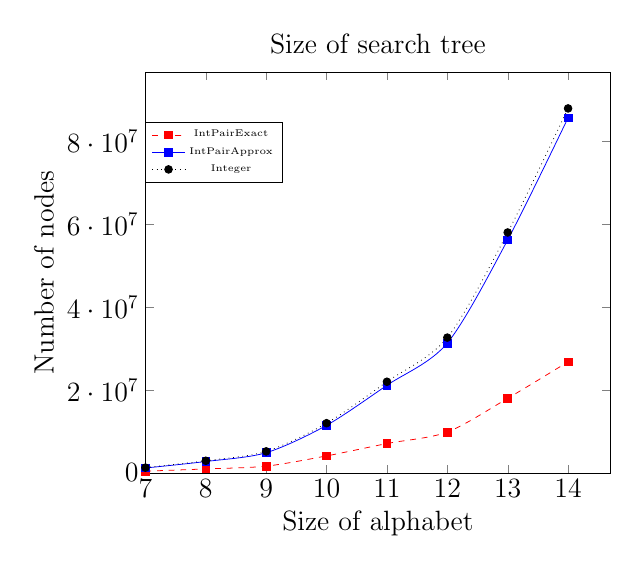
\begin{tikzpicture} [scale=0.7, font=\Large]
    \begin{axis}[
        title=Size of search tree,
        ylabel=Number of nodes,
        xtick=data,
        ymin=0, 
        xlabel=Size of alphabet ]
      \addplot[smooth,mark=square*, mark options={solid},red, dashed]
      coordinates{ (7,427514) (8,969947) (9,1645581) (10,4116333) (11,7102695) (12,9882298) (13,18019942) (14,26841504)
      }; %\label{ie_plot}
      \addlegendentry{IntPairExact}
      \addplot[smooth,mark=square*, mark options={solid},blue]
      coordinates{ (7,1195984) (8,2764047) (9,4887805) (10,11496449) (11,21168309) (12,31364902) (13,56283604) (14,85763254)
      }; %\label{ia_plot}
      \addlegendentry{IntPairApprox}
      \addplot[smooth,mark=*,mark options={solid},black, dotted]
      coordinates{ (7,1283617) (8,2939856) (9,5206922) (10,12012764) (11,22020396) (12,32681442) (13,58068844) (14,88024314)
      }; %\label{int_plot}
      \addlegendentry{Integer}
    \end{axis}
  \end{tikzpicture}
  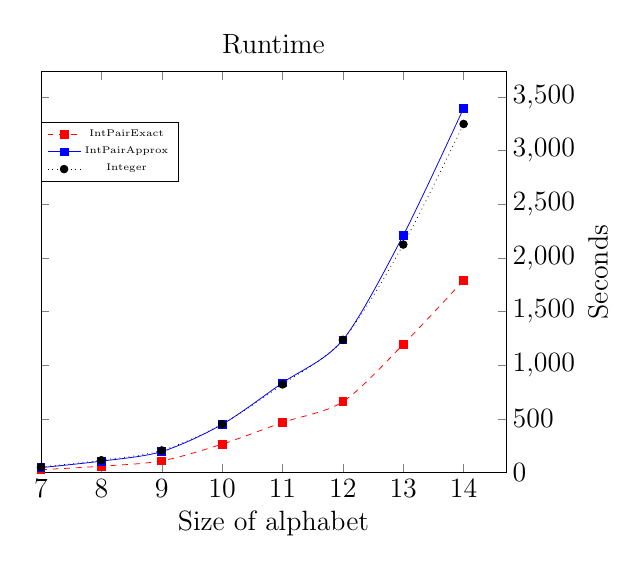
\begin{tikzpicture} [scale=0.7, font=\Large]
    \begin{axis}[
        yticklabel pos=right,
        xtick=data,
        title=Runtime,
        ylabel=Seconds,
        xlabel=Size of alphabet,
        ymin=0, ]
      \addplot[smooth,mark=square*,mark options={solid},red, dashed]
      coordinates{ (7, 27.559) (8, 59.866) (9, 109.743) (10, 265.565) (11, 467.290) (12, 660.466) (13, 1194.665) (14, 1791.396)
      };% \label{IntPairExact Run}
      \addplot[smooth,mark=square*,mark options={solid},blue]
      coordinates{ (7, 46.890) (8, 107.237) (9, 196.052) (10, 449.382) (11, 836.755) (12, 1237.011) (13, 2210.994) (14, 3395.879)
      }; %\label{IntPairApprox Run}
      \addplot[smooth,mark=*,mark options={solid},black, dotted]
      coordinates{ (7, 51.783) (8, 115.192) (9, 206.274) (10, 452.126) (11, 822.169) (12, 1237.290) (13, 2125.013) (14, 3248.002)
      }; %\label{IntegerRun}
      \addlegendentry{IntPairExact}
      \addlegendentry{IntPairApprox}
      \addlegendentry{Integer}
    \end{axis}
  \end{tikzpicture}

%  \begin{tikzpicture}[scale=1.4]
%    \draw[very thick] (-4,0) -- (4,0);
%    \draw[draw=white] (-5,-0.2) -- (5,-0.2);
%  \end{tikzpicture}


%  \begin{tikzpicture} [scale=0.8]
%    \begin{semilogyaxis}[
%        title=No nodes logarithmic scale,
%        ylabel=nodes,
%        xtick=data,
%        ymin=0, 
%        xlabel=symbols ]
%     \addplot[smooth,mark=square*, mark options={solid},red, dashed]
%      coordinates{ (7,427514) (8,969947) (9,1645581) (10,4116333) (11,7102695) (12,9882298) (13,18019942) (14,26841504)
%      }; %\label{ie_plot}
%      \addlegendentry{IntPairExact}
%      \addplot[smooth,mark=square*, mark options={solid},blue]
%      coordinates{ (7,1195984) (8,2764047) (9,4887805) (10,11496449) (11,21168309) (12,31364902) (13,56283604) (14,85763254)
%      }; %\label{ia_plot}
%      \addlegendentry{IntPairApprox}
%      \addplot[smooth,mark=*,mark options={solid},black, dotted]
%      coordinates{ (7,1283617) (8,2939856) (9,5206922) (10,12012764) (11,22020396) (12,32681442) (13,58068844) (14,88024314)
%      }; %\label{int_plot}
%      \addlegendentry{Integer}

%    \end{semilogyaxis}
%  \end{tikzpicture}
%  \begin{tikzpicture} [scale=0.8]
%    \begin{semilogyaxis}[
%        title=Runtime logaritmhic scale,
%        yticklabel pos=right,
%        xtick=data,
%        ylabel=runtime (ms),
%        xlabel=symbols,
%        ymin=0,  ]
%      \addplot[smooth,mark=square*,mark options={solid},red, dashed]
%      coordinates{ (7, 27559) (8, 59866) (9, 109743) (10, 265565) (11, 467290) (12, 660466) (13, 1194665) (14, 1791396)
%      }; %\label{IntPairExact Run}
%      \addplot[smooth,mark=square*,mark options={solid},blue]
%      coordinates{ (7, 46890) (8, 107237) (9, 196052) (10, 449382) (11, 836755) (12, 1237011) (13, 2210994) (14, 3395879)
%     }; %\label{IntPairApprox Run}
%      \addplot[smooth,mark=*,mark options={solid},black, dotted]
%      coordinates{ (7, 51783) (8, 115192) (9, 206274) (10, 452126) (11, 822169) (12, 1237290) (13, 2125013) (14, 3248002)
%      }; %\label{IntegerRun}
%      \addlegendentry{IntPairExact}
%      \addlegendentry{IntPairApprox}
%      \addlegendentry{Integer}
%    \end{semilogyaxis}
%  \end{tikzpicture}
  \caption{Varying the number of symbols. The other parameters are fixed. Number of states=7, max cost per transition=15, and number of steps=7.}\label{fig:symbols}
\end{figure}
